\chapter{Surface current on the waveguide walls}
In this chapter, we will establish that taking a limiting case for the fields for the rectangular waveguide must represent the fields we got for parallel plane waveguides. Now we show that the field we got for a rectangular waveguide can represent the field we got for a parallel plane waveguide in the limiting case when one of the dimensions of the rectangular waveguide becomes infinity. To do this, we ask the question what happens to the mode which was $TM_0$ (or the $TEM$ mode) in the parallel plane waveguide? Does this mode exist inside the rectangular waveguide or only inside a parallel plane waveguide?

Considering the rectangular waveguide, we could find out that the electric and magnetic fields are both perpendicular to the direction of propagation so that the magnetic fields must lie in the XY plane shown in figure~\ref{fig:group4001}. That means they must perform a closed loop in the plane. Then there has to be an electric current enclosed by the magnetic field lines, then and only then can the magnetic field lines survive. Hence there would either be a \textbf{conduction}\index{conduction current} or \textbf{displaccment}\index{displacement current} current that will guarantee the survival of the magnetic field lines since we do not have any conducting medium inside the waveguide\footnote{The waveguide is completely hollow, with pure dielectric inside, and there is no possibility of conduction current enclosed by the magnetic field lines}. Hence conduction current is zero inside the rectangular waveguide and magnetic field lines can only be sustained by the fact that we have a displacement current, and it must be flowing in the z-direction. This displacement current will also require an electric field going in the z direction which will already say is non-existent for $TEM$ mode. Recall we have established that the electric field only lies on the transverse plane for $TEM$ mode. It does not have a component perpendicular to the plane of the paper.
\begin{figure}[h]
\centering
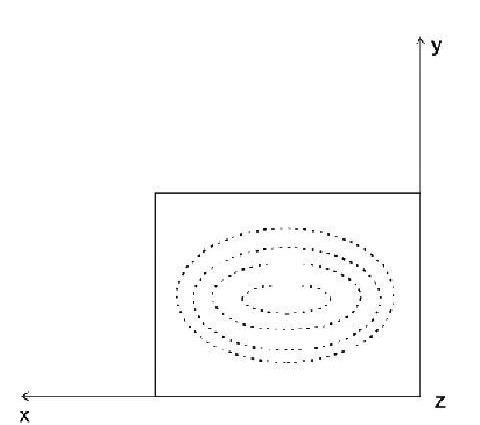
\includegraphics[width=0.6\linewidth]{./graphics/group4001}
\caption{Field patterns of the magnetic fields on the rectangular waveguide wall in the XY plane}
\label{fig:group4001}
\end{figure}

If that is so, we cannot have the displacement current inside the waveguide that is in the z-direction, so either we have a conduction current or displacement current going in the z-direction. Thus, there is no current which is flowing perpendicular to the plane of the paper, and hence there is no current sustaining the magnetic field lines. Based on amperes law, the magnetic field lines must enclose current; hence, these fields lying in the transverse plane cannot exist, as there are no currents to support the magnetic field lines. Thus the $TEM$ cannot exist inside a rectangular waveguide, so $TEM$ mode \textbf{does not exist in} a \textbf{rectangular waveguide}\index{transverse electromagnetic mode}.

\section{Parallel plane waveguide as a limiting case of the rectangular waveguide}
Let us take a parallel plane waveguide as a limiting case of a rectangular waveguide. If we take the rectangular waveguide of dimension width, $a$ and height, $b$ and make ${b=\infty}$, we get a structure shown in figure~\ref{fig:page3} where the wave is travelling in the z-direction. So if the electric field resides in the y-direction and the wave is going to propagate in the z-direction, this would essentially correspond to the $TE$ mode. 
\begin{figure}[h]
\centering
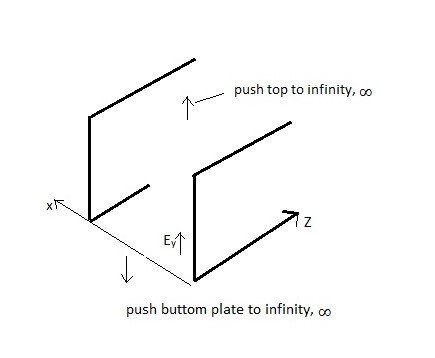
\includegraphics[width=.7\linewidth]{./graphics/page3}
\caption{Parallel plane waveguide as a limiting case of the rectangular waveguide if $b=\infty$}
\label{fig:page3}
\end{figure}

With an electric field in the y-direction as shown in figure~\ref{fig:page3}
\begin{dmath*}
{E_x = E_z = 0 \qquad E_y = - \frac{j\omega\mu a}{\pi} C\sin(\frac{\pi x}{a})e^{-j\beta z}}
\end{dmath*}
\begin{dmath*}
H_x =  \frac{j\beta a}{\pi} C\sin(\dfrac{\pi x}{a})e^{-j\beta z}
\end{dmath*}
\begin{dmath*}
H_y = 0\qquad H_z = C\cos(\dfrac{\pi x}{a})e^{-j\beta z} 
\end{dmath*}
In this case, the magnetic field components ${H_x}$ and ${H_z}$ exist and all these fields were constant as a function of y. 

Something we can get now with ${b=\infty}$ is that there are no boundary conditions to apply in the y direction. The field is infinite, then ${E_y}$ is constant along the y direction. That is precisely the field we got with a parallel plane waveguide. So in a rectangular waveguide, we can take ${TE_{10}}$ mode and make b in infinity and since we do not have any dependence of $E$ with respect to y, it means that the fields in the ${TE_{10}}$ case are essentially the same for a parallel plane waveguide. So the ${TE_1}$ mode of a parallel plane waveguide has essentially the same field as ${TE_{10}}$ mode of a rectangular waveguide. Now we have a magnetic field in the z-direction. 

So in the limiting case of the ${TE_{10}}$ mode,we can get the transverse electric mode, the lowest order transverse electric mode for the rectangular waveguide which is also the lowest order transverse electric mode for the parallel plane waveguide, $TE_1$ mode. Another mode we had was the $TEM$ mode for which the electric field was not tangential to the boundaries,(i.e along the x-axis) the magnetic field was tangential to the boundary (along the y direction) and we say that was the mode in which was not dispersive and travels as if the conducting boundary are not existing and that was the mode which was the $TEM$ mode. The magnetic and electric fields for the parallel plane waveguide for the $TEM$ mode is shown in figure~\ref{fig:page4}. 
\begin{figure}[h]
\centering
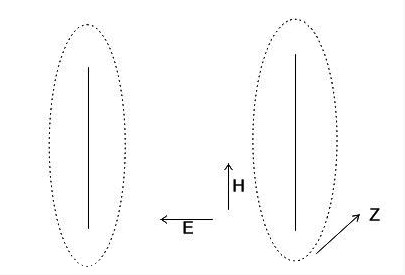
\includegraphics[width=.7\linewidth]{./graphics/page4}
\caption{Field patterns and surface current for the electric and magnetic fields in a parallel plane waveguide in the $TEM$ mode}
\label{fig:page4}
\end{figure}

The wave travels without any variation of the electric and magnetic field as shown because neither the components of the magnetic field require the boundary conditions to be satisfied which is tangential, so we can always have surface currents, nor the normal components of an electric field needs only boundary condition to be satisfied. We can always have the surface charge induced to compensate for the normal component of the electric field. So this mode, the $TEM$ mode, exists inside the parallel plane waveguide.

One can ask the question that if figure~\ref{fig:page4} was the limiting case of the rectangular waveguide, how come the $TEM$ mode exists in the parallel plane waveguide, but not in a rectangular waveguide? We argue that since the magnetic field is in the y direction and the plane is extended in the y direction, the magnetic field lines essentially close at infinity and enclose the conducting walls as shown by dotted lines then these conducting planes have a surface current flowing in them. In the case of the rectangular waveguide where those boundaries are finite, the magnetic fields close up on themselves and thus a current is enclosed. That is why the $TEM$ mode cannot exist in rectangular waveguides but can with a parallel plane structure. The magnetic field lines will close at infinity and enclose the plane conductors as shown in figure~\ref{fig:page4} so the $TEM$ mode can exist inside parallel plane waveguides. This is the mode that propagates in a two-conductor system like coaxial cables.

So whenever we have a two-conductor system, the lowest mode which will propagate will be $TEM$ mode, however, if we go to the rectangular waveguide, the lowest mode which will propagate will be ${TE_{10}}$ mode. The important conclusion to draw is that whenever we have a hollow structure, like a hollow pipe kind of waveguide, the $TEM$ mode cannot exist which is non-dispersive. It is a special mode that is not supported by the rectangular waveguide. That is why we have all the problems of dispersion and so on, inside a rectangular waveguide. The parallel plane waveguide is still a structure which is infinite in extent, it cannot be realized in practice. It is good for understanding, but when we want to realize the structure in practice, it is the rectangular waveguide which is realizable, not the parallel plane waveguide. So whenever we have a physical structure which is a rectangular waveguide, we always have a cut-off frequency associated with that and we always have problems like dispersion and so on associated with them.

\section{Surface current on the parallel plane waveguide walls}
With this understanding, let us try to see the current which gets excited on the walls of the waveguide, which actually supports these fields inside the waveguide. So whether we take a parallel plane or rectangular waveguide, what is the mechanism by which these fields are supported inside the waveguide? what are the sources? The sources are nothing but surface charge and surface currents which lie on the inner surface of the waveguides. So as the wave travels even the surface charge keeps moving i.e accumulating at different locations as we will see later, these charges and surface currents support the electric and magnetic field inside the waveguide which is responsible for carrying power inside the waveguiding structure. So what we do now is first we try to visualize the fields which would be inside the waveguide and then try to visualize how the currents are distributed on the walls of the waveguide, so let us take the simplest case which is the $TEM$ case for a parallel plane waveguide.

\subsection{$TEM$ mode}
In the parallel plane waveguide shown for $TEM$ mode, the electric field $E$ is perpendicular to the plans. With ${E_y = Ce^{-j\beta z}}$ and ${H_x = \dfrac{C}{\eta}e^{-j\beta z}}$, we can visualize these fields. If we tried out how these fields are going to be a function of space and time in the structure. First, we keep time constant and remember all the qualities above are intrinsic functions of time, so ${e^{j\omega t}}$ is implicit in all the terms.
\begin{align*}
E_y = Ce^{-j\beta z}e^{j\omega t}\\
H_x = {\dfrac{C}{\eta}}e^{-j\beta z} e^{j\omega t}
\end{align*}
\begin{figure}[h]
\centering
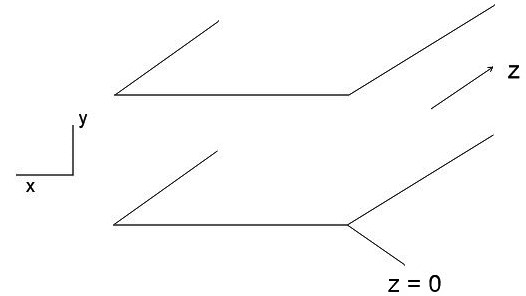
\includegraphics[width=.7\linewidth]{./graphics/page6}
\caption{Parallel Plane waveguide}
\label{fig:page6}
\end{figure}

So these fields are varying as a function of space and time, so if we stand at a particular location in space, the field will vary as a function of time and if we freeze time or say at any instant of time, we look along the waveguide, we see a variation given as $e^{-j\beta z}$. 

So to visualize these fields in 3D, first, we freeze time i.e make ${\omega t}$ constant. At that instant, we want to see how the fields are distributed in space. Once we get those fields distributed in space, then we essentially say that these fields will be moving with a phase velocity for the mode. Then the electric field drifts inside this waveguide with the phase velocity. So when we visualize these fields, essentially we try to visualize the spatial variation of the fields at some instant of time and without losing generality, we can take the time $t=0$, then the field visualization is simply the real part of ${H_y}$ and ${H_x}$ which is ${\mathfrak{Re}\left\{Ce^{-j\beta z}\right\}}$ and ${\mathfrak{Re}\left\{\dfrac{C}{\eta}e^{-j\beta z}\right\}}$. That is ${C\cos\beta z}$ and ${\dfrac{C}{\eta}\cos\beta z}$, if we consider points $z=0$, with variation of ${\beta z}$. So the field varies as a cosine function in the z-direction. It is constant in the XY plane, so we see the cosine variation along the z-direction for these fields. The electric field is the same at any z (i.e XY plane) and in the y-direction.
\begin{figure}[h]
\centering
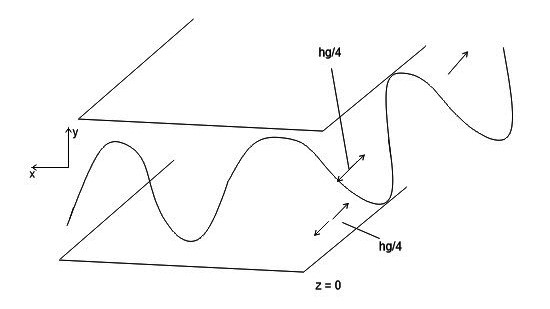
\includegraphics[width=.7\linewidth]{./graphics/group4002}
\caption{Variation of the electric and magnetic field in a parallel plane waveguide}
\label{fig:group4002}
\end{figure}
\begin{figure}[h]
\centering
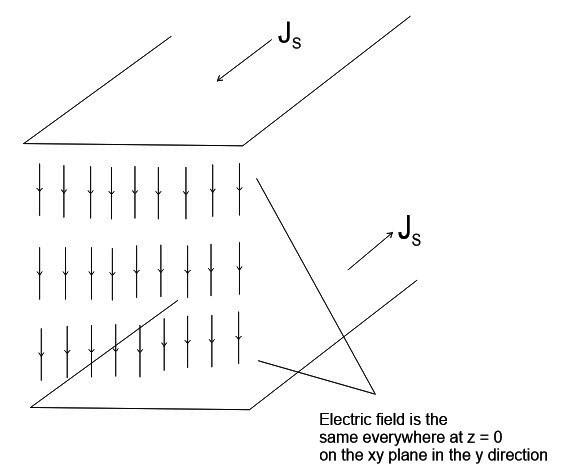
\includegraphics[width=.7\linewidth]{./graphics/page702}
\caption{Surface currents on the walls of the parallel plane waveguide in the $TEM$ mode}
\label{fig:page702}
\end{figure}
\begin{figure}[h]
\centering
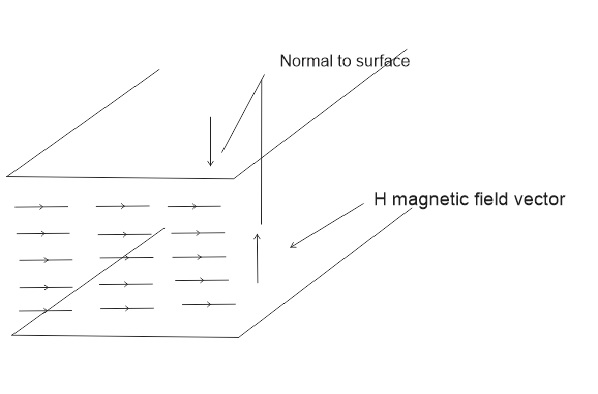
\includegraphics[width=.7\linewidth]{./graphics/page703}
\caption{Magnetic field variation showing normal to parallel plane waveguide surface}
\label{fig:page703}
\end{figure}

The magnetic field is the same at z (XY plane) and in the x-direction. The $E$ and $H$ direction is maintained to show the direction of propagation by the Poynting theorem\footnote{a theorem proposed by a British physicist named John Henry Poynting}. So $E$ starts maximum while $H$ is maximum at $z=0$, at ${z= \dfrac{\lambda_g}{4}}$ they have reduced to zero. Beyond ${z= \dfrac{\lambda_g}{4}}$, they change direction and start increasing till they go to another maximum at ${z=\dfrac{\lambda_g}{2}}$. They again start decreasing from the direction of ${z=\dfrac{\lambda_g}{2}}$ to ${z=\dfrac{3\lambda_g}{4}}$ where $E$ and $H$ are zero. Beyond ${z=\dfrac{3\lambda_g}{4}}$,  they change direction once more and start increasing getting to $z=0$ state at ${\lambda g}$. With little practice, one can see how the electric and magnetic field varies inside the waveguide. Now we know that if the magnetic field pattern is, as shown in figure~\ref{fig:group4002}, the current which is going to flow in the surface of the conductor is related to the magnetic fields i.e the tangential component of the magnetic fields. The ${\hat{n}\times\bar{H}}$ gives the surface currents on the conducting walls. Since we are considering here ideal conductors, essentially, calculating ${\hat{n}\times\bar{H}}$, that is the current which is truly confirmed to the surface of this parallel plane waveguide. 

The normal to the surface of $H$ fields is shown in figure~\ref{fig:page703}. We choose the normal pointing inwards as that is the part that bounds the electromagnetic wave to be propagated. The normal opposite that would be the electromagnetic wave was propagated outside the conducting plane. So the unit vector of the wave plane is going upward in ${\hat{y}}$ direction for the upper plane in ${-\hat{y}}$ direction. Now we can calculate ${\hat{n}\times\bar{H}}$. The ${\hat{n}\times\bar{H}}$ will give the direction of surface current, which top plane, ${\hat{n}\times\bar{H}}$ is the negative z-direction as to say the surface current is coming out from the top plane and going in the bottom plane. Hence ${J_s}$ direction is shown on the top and bottom plane respectively. ${J_s}$ will be having the same variation as the variation of the magnetic field. Maximum at $z=0$, and ${z= \dfrac{\lambda_g}{4}}$. Maximum at ${z=\dfrac{\lambda_g}{2}}$ but with direction reversed, zero at ${\dfrac{3\lambda_g}{4}}$ and maximum again at ${z=\lambda_g}$ with the same direction as with $z=0$. 

So in a two-conductor system, we get current to flow in the direction in which the wave is propagating. ${J_s}$ in the positive z-direction in the bottom at $z=0$ and ${J_s}$ in the negative z-direction at the top for $z=0$. If we have a two-conductor system like the coaxial cable, we connect a voltage source, current goes inside the conductor and returns back through what is called a ground path. So we see that the current goes inside from one terminal and comes outside from the other terminal. So in that situation of the two-conductor system, the direction of the current flow which we have for the $TEM$ mode (keep in mind) is the same as the direction of wave propagation. So the current is going from the bottom plane and returning from the top plane at $z=0$. The question we ask is if the wave is propagating in the z-direction, is it always true that current has to flow in the z-direction or the direction of wave propagation? Then we got the answer which is wrong. That is because we always discuss the transverse electromagnetic mode.

The fact that we are used when we go to the low-frequency circuit, immediately we jump to the conclusion that yes since the wave is moving in the z-direction, the power is flowing in the z-direction, and the current must flow in that direction.

\subsection{$TE$ mode}\index{transverse electric mode}
\begin{figure}[h]
\centering
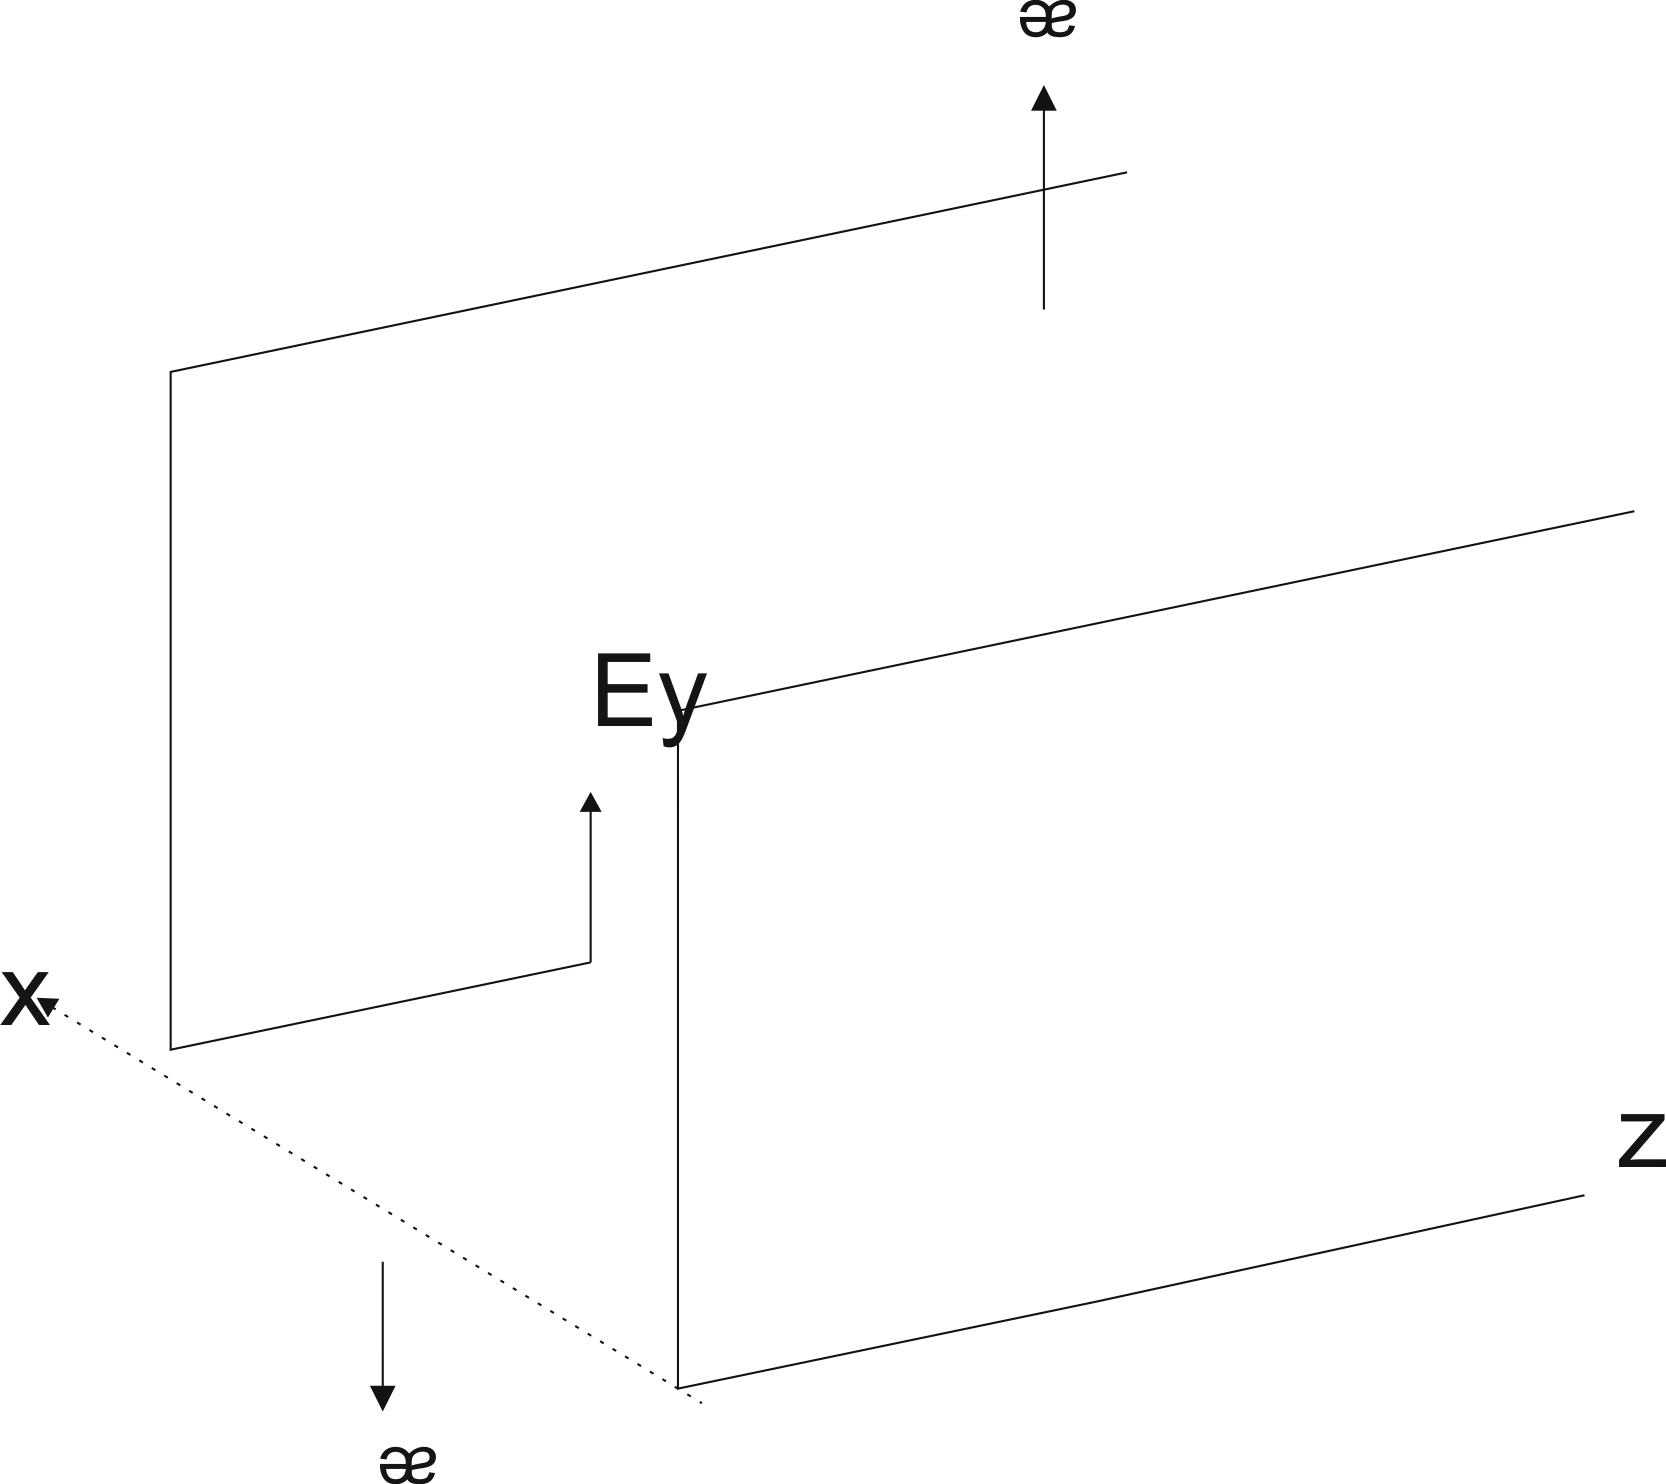
\includegraphics[width=.7\linewidth]{./graphics/WATSON4}
\caption{Analysis of parallel plane waveguide propagating wave in the $TE$ mode}
\end{figure}

Let us look at the parallel plane waveguide considering the $TE$ mode and let us see what will be the direction of the current and field in the waveguide. As we saw, the fields for the parallel plane waveguide are identical to the $TE_{10}$ mode for rectangular waveguide giving as
\begin{align*}
E_x &= E_z = H_y = 0\\
E_y &= -\dfrac{j\omega \mu a}{\pi}C\sin(\dfrac{\pi x}{a})e^{-j\beta z}\\
H_x &= -\dfrac{j\beta a}{\pi}C\sin(\dfrac{\pi x}{a})e^{-j\beta z}\\
H_z &= C\cos(\dfrac{\pi x}{a})e^{-j\beta z}
\end{align*}
So the electric field will be y oriented, and it will have a variation which would be in the z-direction with the value of ${\beta}$. To visualize ${E_y}$, let's take the real part of ${E_y}$ and look at its variation with respect to x,y and z. This will give us a 3-dimensional picture of the fields.
\begin{dmath*}
E_y = \dfrac{-j\omega \mu a}{\pi}C\sin(\dfrac{\pi x}{a})e^{
-j\beta z}\equiv e^{-j\dfrac{\pi}{2}}\times\dfrac{\omega \mu a}{\pi}C\sin(\dfrac{\pi x}{a})e^{-j\beta z}  = \dfrac{\omega \mu a}{\pi}C\sin(\dfrac{\pi x}{a})e^{-j\left(\beta z + \dfrac{\pi}{2}\right)
}
\end{dmath*}
\begin{dmath*}
\mathfrak{Re}\left\{E_y\right\} = \dfrac{\omega \mu a}{a}C\sin(\dfrac{\pi x}{a})\cos(\beta z + \dfrac{\pi}{2})
\end{dmath*}
Recall, $\cos(-\left(\beta z + \dfrac{\pi}{2}\right))=\cos(\beta z + \frac{\pi}{2})$, i.e. cosine is an even function and let ${\dfrac{\omega \mu aC}{\pi}\equiv A}$, thus we have 
\begin{dmath*}
\mathfrak{Re}\left\{E_y\right\} = A\sin(\dfrac{\pi x}{a})\cos(\beta z +\dfrac{\pi}{2}) = A\sin(\dfrac{\pi x}{a})\sin(\beta z) = A\sin(\dfrac{\pi x}{a})\sin(\dfrac{2\pi z}{\lambda_g})
\end{dmath*}
We can do the same for ${H}$
\begin{align*}
\mathfrak{Re}\left\{H_x\right\} = B\sin(\dfrac{\pi x}{a})\sin(\dfrac{2\pi z}{\lambda_g})\\
\mathfrak{Re}\left\{H_z\right\}= C\cos(\dfrac{\pi x}{a})\cos(\dfrac{2\pi z}{\lambda_g})
\end{align*}
These are the field which is in existence when time is fixed, say at $t=0$. At that instant, these three expressions give the fields along the waveguides. As we can see in the z-direction, the fields are all sinusoidal with a spatial period of ${\lambda_g}$. However ${\mathfrak{Re}\left\{H_z\right\}}$ and ${\mathfrak{Re}\left\{H_z\right\}}$ are in \textbf{quadrature}, that is ${90^{o}}$ degree out of phase with each other so that when ${H_x}$ is maximum, ${H_z}$ is zero. And when ${H_z}$ is maximum, ${H_x}$ is zero. 

So in space, we have two components, the ${H_x}$ and the ${H_z}$ components. ${H_x}$ component has sine variation along z. With $z=0$, ${H_x}$ is zero at that location, but ${H_z}$ is maximum at that location. If we go ${z=\dfrac{\lambda_g}{4}}$, ${H_x}$ is maximum and ${H_x=0}$.

From the top of this parallel plane waveguide, we see the magnetic fields as shown in figure~\ref{}. Since the magnetic field is close to themselves, it is only a matter of imagination. To close the magnetic field loops as shown by the dotted lines ${\dfrac{\lambda_g}{4}}$ from here the direction with reverse to have the dotted line from $\dfrac{\lambda_g}{4}$  to $\dfrac{\lambda_g}{2}$ and so on.
\begin{figure}[h]
\centering
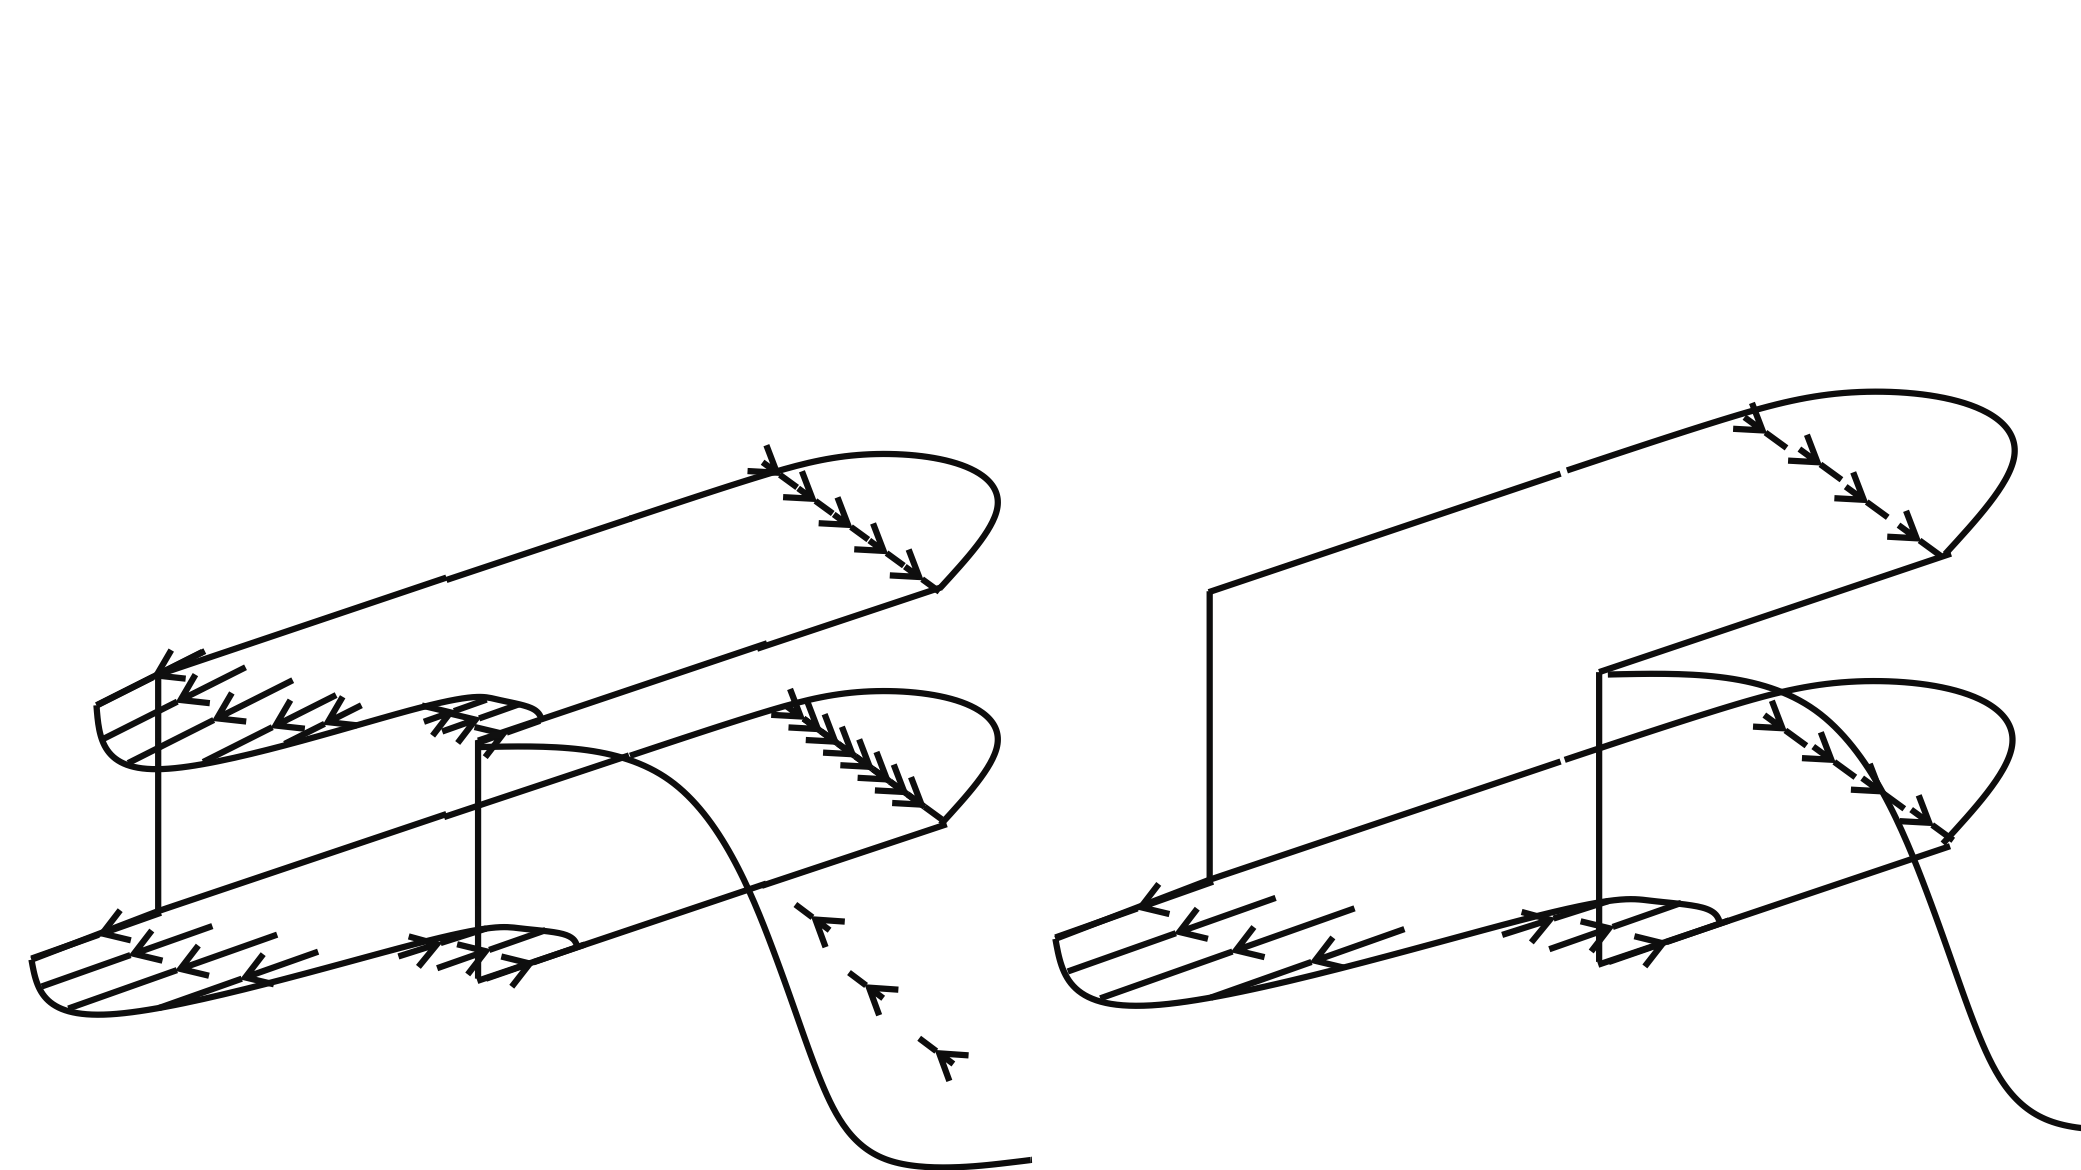
\includegraphics[width=1\linewidth]{./graphics/WATSON}
\caption{Magnetic field patterns in the parallel plane waveguide operating in the $TE$ mode}
\label{fig:watson}
\end{figure}

Hence we can complete this to get the field distribution shown in figure~\ref{fig:watson}, for a waveguide going from ${-\infty}$ to ${+\infty}$. So from the top in a parallel plane waveguide, the magnetic field lines look like rolled carpets which are scattered inside the structure. They are of infinite length perpendicular to the plane of the paper. This is how the magnetic field will be distributed.

However for the electric field, ${E_y= A\sin(\dfrac{\pi x}{a})\sin(\dfrac{2\pi z}{\lambda_g})}$ the electric field has variation in the z-direction since as ${H_x}$, but it is oriented in the y direction. So from the top, the electric field lines is perpendicular to the plane of the paper. The behaviour of ${E_y}$ and ${H_x}$ is identical, that means whenever ${H_x}$ is maximum, ${H_y}$ will be maximum. So it has identical variation to ${H_x}$. So if we look at the ${H_x}$ component, so the electric field is maximum at ${z= \dfrac{\lambda_g}{4}}$ and minimum at $z=0$ with the ${H_x}$ variation along z. The electric field always points in the y direction with wave propagating in the z direction and ${H_x}$ in the x direction, ${H_y}$ from ${E\times H= \hat{z}}$ must point in the y direction at that point.

So we have a certain notion we have we have built for an electrical circuit that is essentially from the transverse nature of the electromagnetic wave. As soon as we make the departure from a transverse electromagnetic wave to a transverse electric or transverse magnetic case, all those notions completely break down and we get a much clearer picture of the propagation of electromagnetic waves and the current and the distribution of charges and so on for various configurations. So with this understanding of the current flow for a parallel plane structure which is rather the simplest structure, now we can discuss the field distribution inside a rectangular waveguide which is a more practical structure.

In summary, we saw that the $TEM$ mode cannot exist inside a rectangular waveguide. We also showed that by taking limits with a rectangular waveguide and pushing one of the dimensions to infinity, then the field we get for a rectangular waveguide is identical to what we have got for a parallel plane waveguide. Then we developed a mechanism for visualizing these fields inside a waveguide. We saw two cases, one was of the transverse electromagnetic wave in a parallel plane waveguide, and the other was the ${TE_1}$ mode inside the parallel plane waveguide. 
